\subsection{Parallelization}
In this section we will describe a set of transformation rules known as Parallelizations. In \cref{fig:trivial-example} we use only the exact number of modules necessary to produce the three recipes given in \cref{fig:toy-recipes}. It could easily be imagined that we had more modules capable of doing the same work as the ones in \cref{fig:trivial-example}. As such we produce a set of transformation rules that allow for possible greater throughput by parallelizing free modules with similar modules already in a line.


\subsubsection{$Para_0$: Parallelization Between Common Modules}
We start by defining the most common type of parallelization with the $Para_0$ transformation rule. Informally the rule states that if we have the total order $M_{s,e}$ of modules in between the modules $s$ and $e$. Then we can add a parallel line starting at $s$ and ending at $e$, if we can find an existing total order of free modules $P_{s,e}$ that can perform the same work as the modules in $M_{s,e}$. The visual representation of the $Para_0$ transformation rule can be seen \cref{fig:para0}. Here we expand the visual representation of our rules with the square box with a T in it. This box is just represents a single module that can perform no work, commonly referred to as a transport module.

\begin{figure}[H]
	\centering
	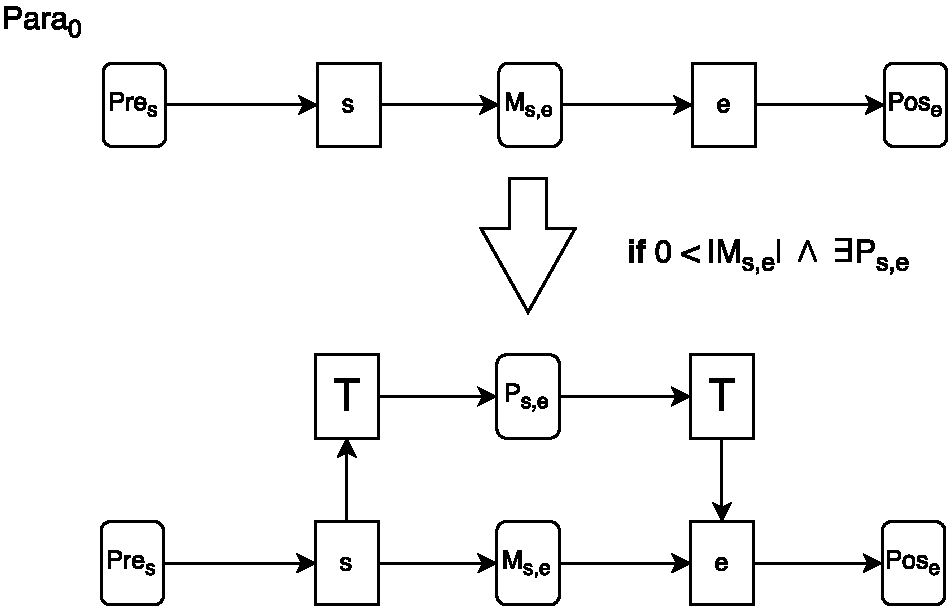
\includegraphics[width=0.7\textwidth]{para0.pdf}
	\caption{A visual representation of the $Para_0$ transformation rule}
	\label{fig:para0}
\end{figure}

In order to find the total order, $P_{s,e,}$, that can perform the same work as $M_{s,e}$. We first define the set of all free modules, $FM$. We say that the set of all free modules is the relative complement of all modules and all modules in a line $\gamma \in \Gamma$.

\[FM = M \setminus \{m | m \in \gamma \land \gamma \in \Gamma\}\]

We then describe a set of pairs of free modules and modules in between $s$ and $e$, where the free module $m$ can at least do the same work as the module in between $s$ and $e$ is currently doing.

\[ParaMap_{s, e} = \{(m, m')| m \in FM \land m' \in M_{s,e} \land AW(m') \subseteq m\} \]

We then describe all sets of pairs that could be a possible parallel line for the modules between $s$ and $e$. Note that this set could be the empty set, as the modules needed for creating a possible line might not available in $FM$.

\[ParaMapPaths_{s,e} = \{p \in ParaMap_{s,e}^2 | (m,m') \in p \land (n,n') \in p \land |p| = |M_{s,e}| \land  \forall m': m' \neq n' \}\]

After this we define $s[1]$ as the operation that given a set of pairs $s$, gives the set of all the first elements of the pairs in $s$.
\[s[1] = \{m_1 | (m_1, m_2) \in s\}\]

Using this we define the total order $P_{s,e}$ as:

\[ P_{s,e} = (p[1], \prec), \texttt{ where } p \in ParaMapPaths_{s,e} \]

This definition means that there might not exist any $P_{s,e}$ at all, or that there might be multiple candidates for $P_{s,e}$.

\subsubsection{$Para_1$: Parallelization without forking module}

\begin{figure}[H]
	\centering
	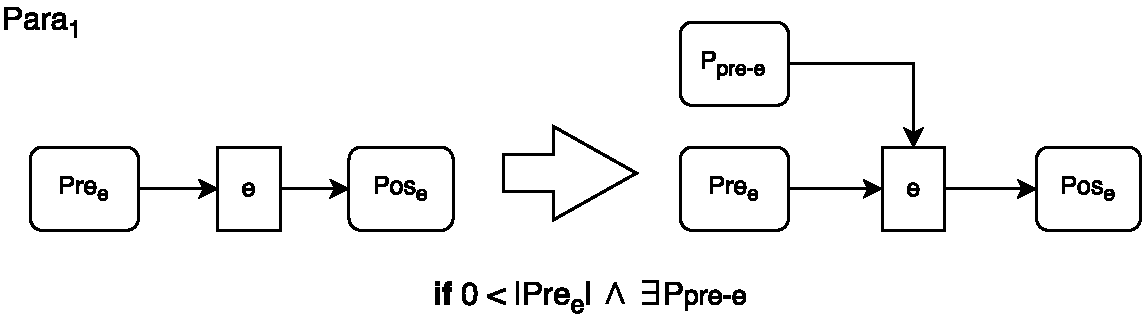
\includegraphics[width=0.8\textwidth]{para1.pdf}
	\caption{A visual representation of the $Para_1$ transformation rule}
	\label{fig:para1}
\end{figure}

\subsubsection{$Para_2$: Parallelization without joining module}


We also have two other cases, one in which we have no end module, meaning that we will fork out a parallel line, and the case where we have no start, meaning we will join in a parallel line. A graph showing both of these cases can be seen respectively in \cref{fig:para_we} and \cref{fig:para_ws}. For the case without start we connect the last module in the total order $(P_{s,e}, <_p)$ to $e$, and for the case without end we connect $s$ to the first module the in the total order $(P_{s,e}, <_p)$.


\begin{figure}[h]
\centering
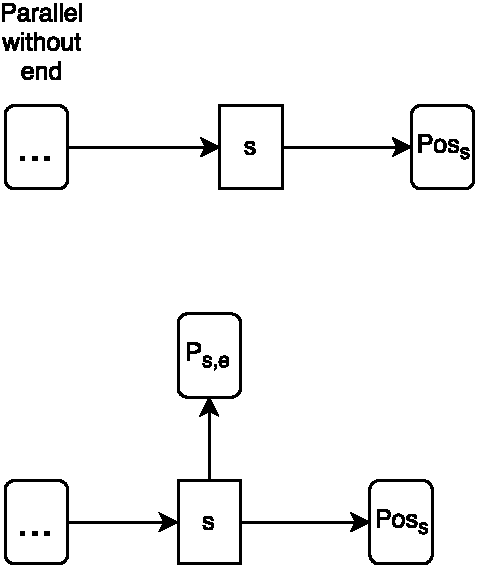
\includegraphics[width=0.3\textwidth]{para_we.pdf}
\caption{Parallelization rule when you do not have an end module}
\label{fig:para_we}
\end{figure}

\begin{figure}[h]
\centering
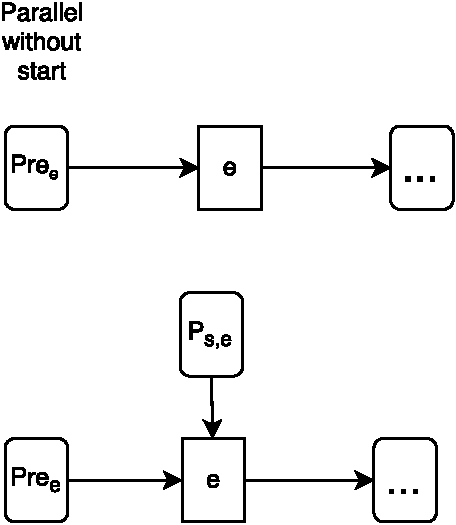
\includegraphics[width=0.3\textwidth]{para_ws.pdf}
\caption{Parallelization rule when you do not have a start module}
\label{fig:para_ws}
\end{figure}

